\documentclass{standalone}
\usepackage{tikz}
\begin{document}
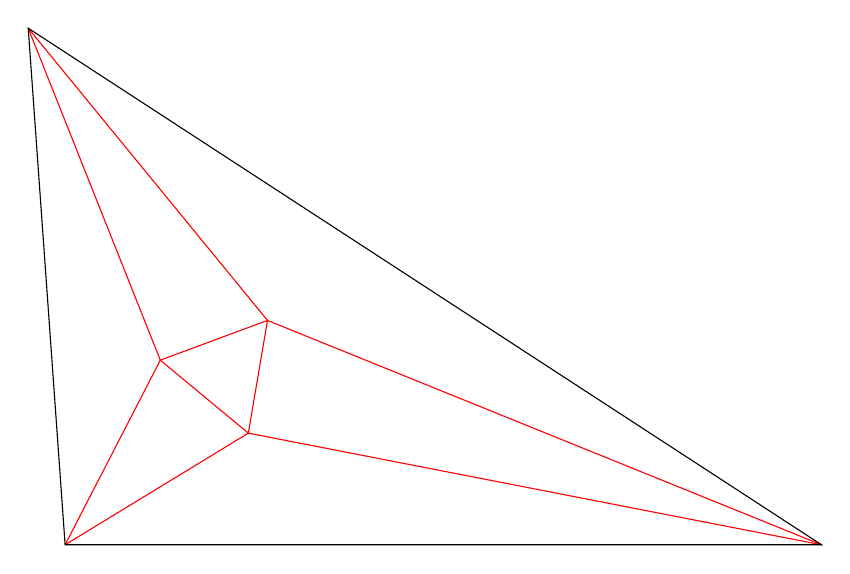
\begin{tikzpicture}[x=1pt,y=1pt]
\draw[red] (54.40,-126.61) -- (86.20,-152.98) -- (93.13,-112.25) -- cycle;
\draw[red] (293.33,-193.33) -- (86.21,-152.98);
\draw[red] (6.67,-6.67) -- (54.40,-126.61);
\draw[red] (93.14,-112.26) -- (293.33,-193.33);
\draw[red] (6.67,-6.67) -- (93.14,-112.26);
\draw[red] (54.40,-126.61) -- (20.00,-193.33);
\draw[red] (20.00,-193.33) -- (86.21,-152.98);
\draw (293.33,-193.33) -- (6.67,-6.67) -- (20.00,-193.33) -- cycle;
\end{tikzpicture}
\end{document}
